\section{Einleitung}

Der Hierholzeralgorithmus findet Eulerkreise in einem vollständigen, ungerichteten Graphen, dessen Knotengrade gerade sind. Im folgenden wird seine Implementierung, sowie sein Laufzeit- und Energieverbrauchsverhalten besprochen.

\section{Hierholzer Laufzeit}

Es wurden drei Messungen durchgeführt. Mit 3.000, 400.000 und 1.000.000 Kanten wurde der Hierholzer-Algorithmus jeweils zehnmal ausgeführt und dabei die Zeit in ms und der Energieverbrauch in Joule mit Hilfe des Commandlinetools PowerLog3.0 von Intel erfasst. Für die einzelnen Messungen ergeben sich folgende grobe Durchschnittswerte:\\
\\
\begin{tabular}[h]{lcr}
Kantenzahl & Zeit in ms & Energieverbrauch in J \\
3000 & 10 & 0.5 \\
400000 & 1300 & 50 \\
1000000 & 5500 & 200 \\
\end{tabular}
\\

\begin{figure}[htbp]
	\centering
		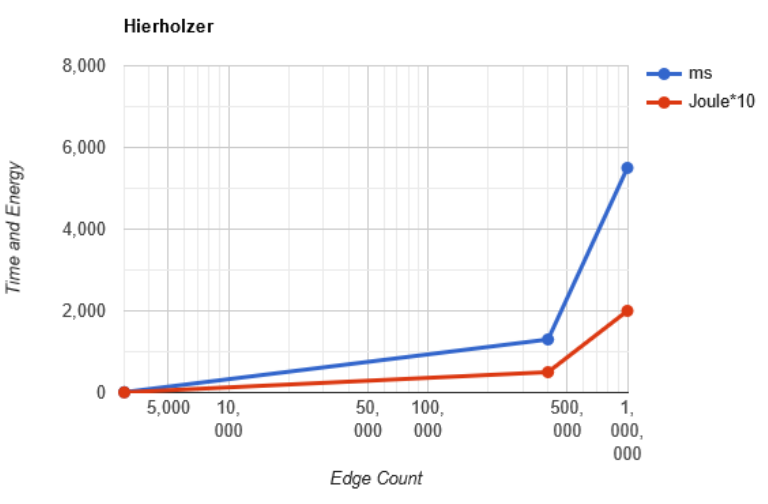
\includegraphics[width=0.6\textwidth]{Latex/Figs/TimeEnergyChart.png}		
	\caption{Verhalten von Zeit und Energie zu Kantenzahl (log)}
	\label{fig:TimeEnergyChart}
\end{figure}

Es ist zu erkennen, dass der Energieverbrauch weniger steil mit der Anzahl der Kanten wächst, als der Zeitaufwand. Aber auf Grund der undurchsichtigen Art und Weise, wie PowerLog3.0 den Energieverbrauch erfasst und der hohen Anzahl an Faktoren, die diesen beeinflussen (Speichertakt, RAM-Spannung, Netzteil, CPU-Takt, Core-Spannung, Festplattenbauart, etc.), kann nur vermutet werden, dass diese gemessenen Werte der Realität entsprechen. Anscheinend kann der Prozessor mit wachsender Zahl an Berechnungen gleicher Art, effizienter umgehen, als mit häufiger wechselnden Berechnungsarten. Dies ist aber nur eine Mutmaßung und eine professionelle Beurteilung der Messung ist auf unserem Fachwissen fußend nicht möglich.\\


\section{Hierholzer Implementierung}

\subsection{Schritte}

Zunächst wird eine ArrayList mit den Knoten der Eulerkreise circleNodes deklariert.
Die folgenden Schritte werden solange wiederholt, bis im Graph keine Kanten mehr enthalten sind.\\
\begin{itemize}
    \item I) 
    Wenn die Liste mit den Knoten der Eulerkreise noch leer ist, wird mit dem ersten Knoten aus dem Graph begonnen, sonst mit irgendeinem aus der in der Liste enthaltenen Knoten, der noch erreichbare Nachbarn hat.\\
    \item II) 
    Von diesem Startknoten ausgehend wird nun ein Kreis im Graph gesucht. Dafür werden solange noch unbesuchte Kanten gegangen, bis ein Knoten erreicht ist, der gleich dem Startknoten ist. Um zu überprüfen, ob eine Kante schon besucht wurde, werden solche in einem Hashset visitedEdges, welches zu Beginn einer jeden Iteration geleert wird, zwischengespeichert.\\
    \item III) 
    Wenn der Kreis geschlossen ist, werden die gefundenen Knoten zunächst den circleNodes und dann als Graphobject  zusammengefügt der Ergebnisliste hinzugefügt, dann die visitedEdges, nach einer für die späteren Verwendung des Graphobjetkts notwendiger Zwischenspeicherung cachedEdges, aus dem Graphen entfernt.\\
    \item IV)
    Nun wird wieder mit Schritt I) begonnen, wenn der Graph noch Kanten enthält.
    \item V) 
    Wenn der Graph keine Kanten mehr enthält, werden diese mit Hilfe der Zwischenspeicherung cachedEdges wieder dem Graph hinzugefügt. Die Ergebnisliste, bestehend aus den einzelnen Eulerkreisen als Graphobjekte, wird von der Funktion zurückgegeben.
    
\end{itemize}

\subsection{Datentypen}

Zur Ausführung des Hierholzer-Algorithmus müssen verschiedene Objekte wie Kanten und Knoten zwischengespeichert werden. Prüfungen, ob ein Element in einer Datensammlung enthalten ist, hat beim Hashset, anders als bei Listen, eine konstante Komplexität. Deshalb werden die visitedEdges als solches deklariert. 
Eine Arraylist ist grundsätzlich schneller als eine Linkedlist, es sei denn, es werden oft Elemente hinzugefügt. Dann nämlich sorgt die Implementierung von Java dafür, dass das ganze Array auf einen neuen größeren Speicherbereich kopiert wird, was viel Zeit kostet.
Deshalb benutzen wir für alle anderen zwischenspeichernden Datensammlungen die LinkedList.

\subsection{Testen der ungeraden Knotengerade}

In einem Graphen mit mindestens einem Knoten, welcher einen ungeraden Knotengrad hat, kann der Hierholzer Algorithmus keinen Erfolg haben. Ein Beispiel ist hier\ref{fig:unevenGraph} in den Tests zu finden.\\

Um sicherzustellen, dass dem Algorithmus ein valider Graph übergeben wird, wurde folgende Methode implementiert:

\begin{lstlisting}[language = java, frame = trBL]
private static boolean graphIsValid(Graph graph) {
    ....
    List<Node> nodesWithFalseDegree = graph.nodes()
                            .filter(node -> node.getDegree() % 2 != 0)
                            .collect(Collectors.toList());        
    for(Node node: nodesWithFalseDegree) {
        if(node.getEdgeBetween(node.getId()) == null) {
            return false;
        }
    }
    ...
}
\end{lstlisting}

Um zu prüfen ob Knoten einen ungeraden Kantengrad haben, werden diese Knoten zuerst alle in einer Liste gespeichert. Das ist notwendig, denn durch die genutzte Graphstream Bibliothek ensteht folgendes Problem: Angenommen es existiert ein Graph mit einem Knoten A und zwei Nachbarknoten B und C. Der Knoten A hat eine Schleife. Der Graph ist vollständig - A,B und C sind also alle miteinander verbunden (Abb. \ref{fig:loop}). 

\begin{figure}[htbp]
	\centering
		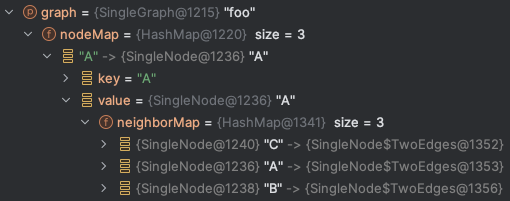
\includegraphics[width=0.6\textwidth]{Latex/Figs/loopedGraphDebugger.png}		
	\caption{Ausschnitt des Graphen mit Loop aus dem Debugger}
	\label{fig:loopedGraphDebugger}
\end{figure}

Wie nun im Debugger zu sehen\ref{fig:loopedGraphDebugger} hat der Knoten A nun nur drei Nachbarn. Zusätzlich hat er auch nur drei adjazente Kanten, AA, AB und AC. Das ist soweit alles korrekt. Der daraus resultierende Knotengrad ist allerdings ungerade und würde diesen Graph als invalide auswerten. Bei Betrachtung des Graphen hat dieser aber einen geraden Knotengrad.\\
Um dieses Problem zu umgehen wird in allen Kanten mit ungeradem Knotengrad also zusätzlich geprüft ob diese Kanten keine Schleifen sind. Erst wenn das der Fall ist, wird der Graph als invalide ausgewertet.

\section{Graphgenerator Implementierung}
Wir haben einen Euler-Multigraphen basierend auf dem vorgeschlagenen Algorithmus erstellt. Gemäß der Anforderung mussten wir einen Multigraphen mit einer festgelegten Anzahl von Knoten und Kanten erstellen. Wir haben eine Überprüfung hinzugefügt, um sicherzustellen, dass die von den Benutzern angegebene Anzahl von Kanten nicht geringer ist als die Anzahl der Knoten. Dies ist unter anderem notwendig, um den Graphen zusammenhängend zu halten. Wir erstellen eine Liste der Knoten des Graphen und eine Liste der Positionen, deren Länge der Anzahl der Kanten entspricht. Wir weisen jeder Knoten eine der Positionen zu. 
Wir speichern in einer HashMap namens posHashMap die Position für jeden Knoten. Zuerst wählen wir aus der posHashMap einen Knoten mit der Positionsnummer 0 oder, falls dieser nicht existiert, weisen wir eine zufällige Knoten als Startknoten zu. Danach iterieren wir von null bis zur Anzahl der Kanten.\\
Wir müssen die actualSource und actualTarget Knoten bestimmen, zwischen ihnen Kanten erstellen und die nächste neue actualTarget-Knoten suchen und die vorherige Zielknoten der Variable actualSource zuweisen. Dies wird in der Funktion getNextNode() implementiert. Eine wichtige Ergänzung zum vorgegebenen Pseudocode wurde eingeführt: Bis wir die Anzahl der Knoten in den Iterationen nicht überschreiten, verwenden wir nicht die Funktion getNextNode(), die Knoten zufällig auswählt, falls sie nicht in posHashMap vorhanden sind. Stattdessen entnehmen wir der Reihe nach Knoten aus der Knotenliste, nachdem wir diese Liste zuvor gemischt haben. Auf diese Weise stellen wir sicher, dass alle Knoten gewählt werden und der Graph zusammenhängend bleibt. Wir verbinden beim Erreichen der vorletzten Kantennummer den aktuellen Knoten mit dem Startknoten, um den Kreis zu schließen.\\
